\section{Feature: Effective Semantic Isomers}

We now shift to examine the failure of surficial distillation: similar conceptual atoms can be linked by different bonds, producing completely different reasoning chains. We call these as \textbf{Semantic Isomers}. Mathematically, a semantic isomer of \(\mathcal{D}\) is any \(\mathcal{D}'\) whose \((P_{\mathcal{D}'}, \pi_{\mathcal{D}'})\) lies near \((P_{\mathcal{D}}, \pi_{\mathcal{D}})\) under a suitable divergence \(D(\cdot \,\|\, \cdot)\). Then, we will analyze how they form, are learned, and sometimes destabilize in Long CoT.


\subsection{Bond structure of Semantic Isomers is the key to Long-CoT learning}

\paragraph{\textbf{Well-structured Semantic Isomers can be effective for Long-CoT learning.}}
To assess whether well-structured Semantic Isomers can enhance Long-CoT learning, we constructed a Long CoT dataset by distilling from advanced reasoning LLMs. As shown in Table~\ref{tab:distill_result}, models exhibit consistent performance gains when trained on these variants (distribution correlation $\thicksim$0.9). This suggests that, within a certain range, multiple effective “allotropic”
variants of reasoning keys can exist.\vspace{-8pt}



\paragraph{\textbf{The model has multiple effective Semantic Isomers, and slight differences can significantly affect the results.}}
As shown in Table~\ref{tab:distill_result}, the structural correlation between R1- and OSS-derived chains can reach 0.95, yet for some models performance with R1-based chains drops by more than 10\%.
This gap indicates the presence of multiple near-optimal Semantic Isomers that are nonetheless fragile, where small changes in the distribution can cause large performance losses.\vspace{-8pt}

\begin{wrapfigure}{r}{0.32\textwidth}
    \centering
    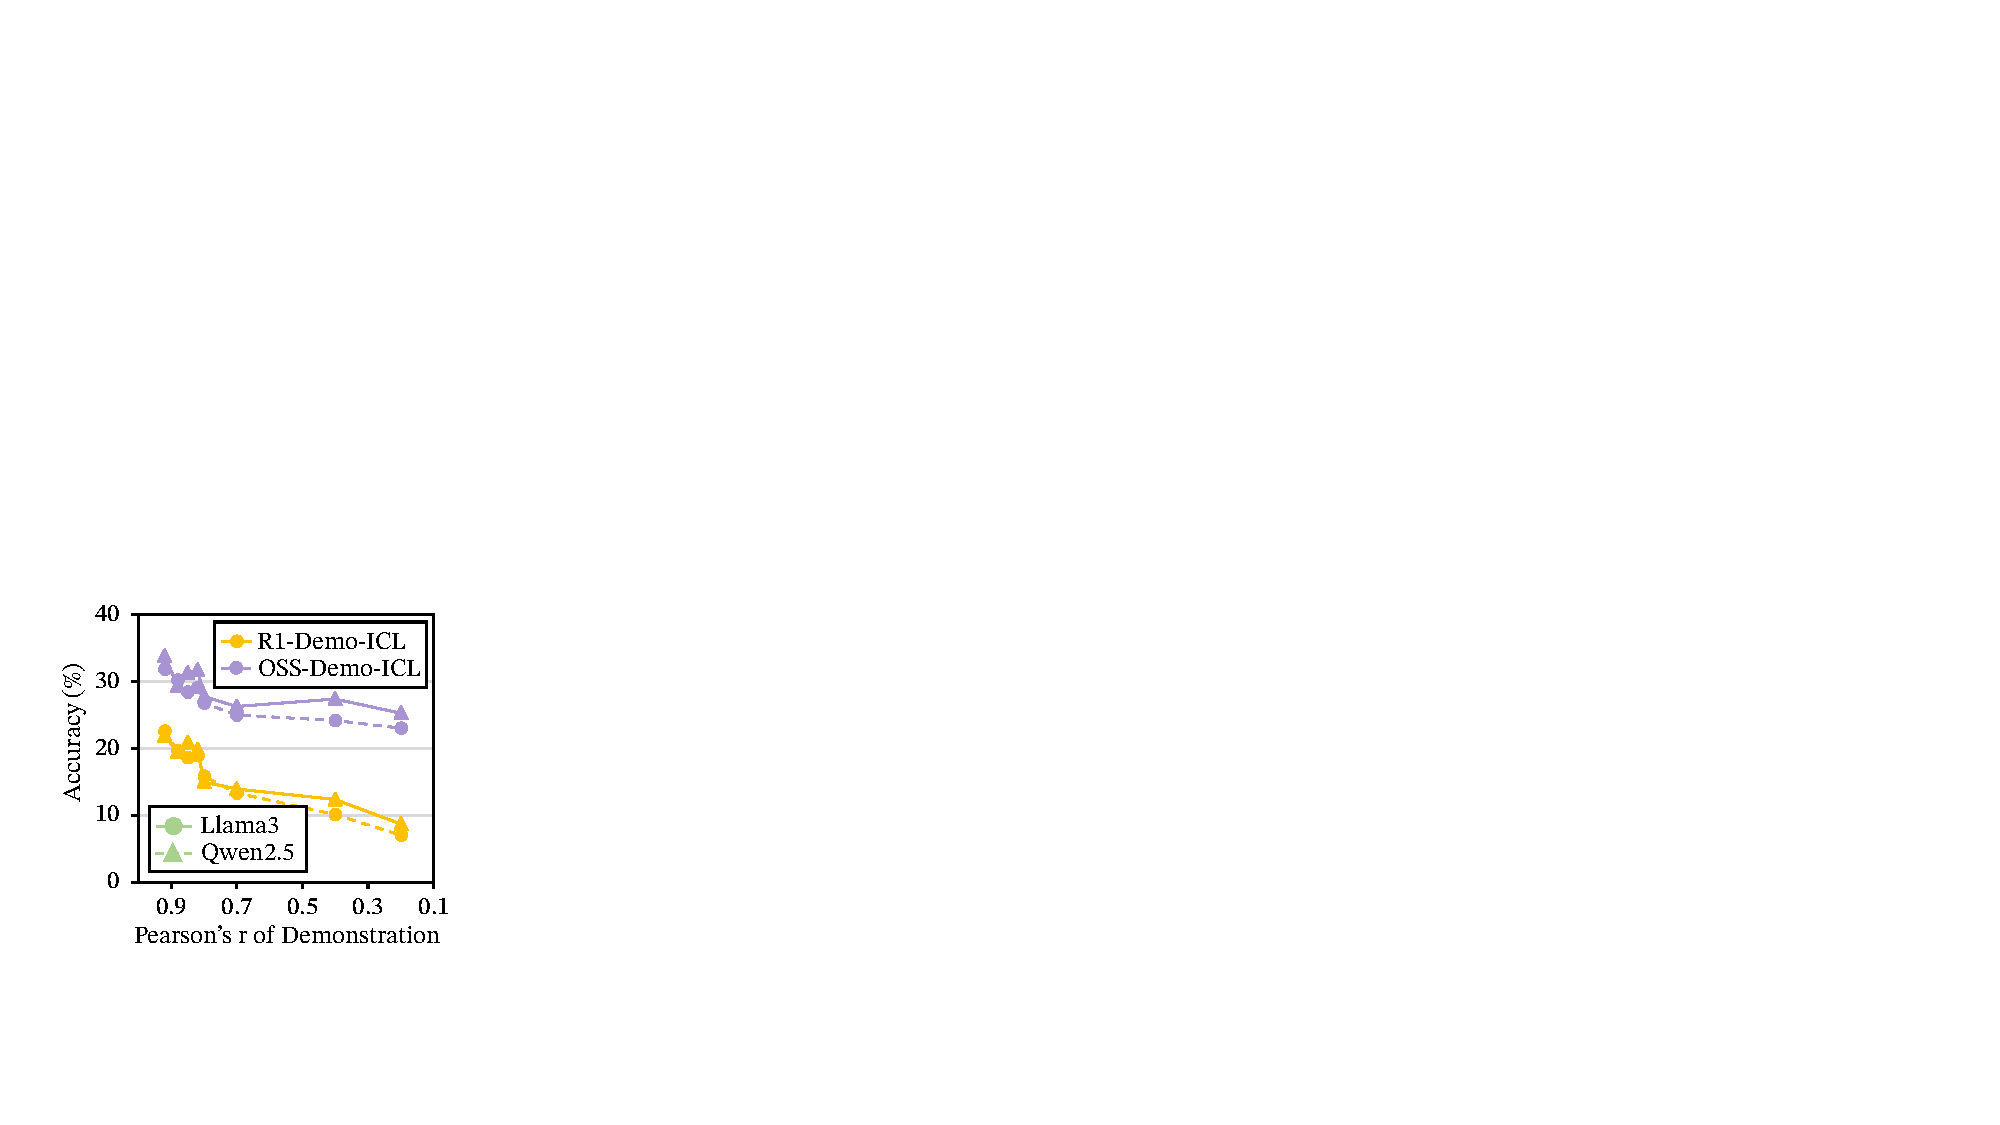
\includegraphics[width=0.30\textwidth]{figures/icl.pdf}
    \caption{The performance of LLama-3.1-8B-Instruction under three different distillation setups from  ICL-augmented Qwen2.5-32B.}
    \vspace{-20pt}
    \label{fig:icl}
\end{wrapfigure}
\paragraph{\textbf{Simulating effective Semantic Isomer structures is the key to ICL distillation.}}
We analyze three ICL setups to simulate Long CoT chains by Qwen2.5-32B-Instruct: demonstrations chosen at random; demonstrations with closely aligned reasoning-key distributions (correlation \(\thicksim\)0.9); and demonstrations with clearly mismatched distributions (correlation \(< 0.8\)). As shown in Fig.~\ref{fig:icl}, substantial performance gains emerge only when demonstrations are constructed to match a specific target distribution of reasoning keys, thereby yielding an appropriate “allotrope” of that distribution.




\begin{figure*}[t]
    \centering
    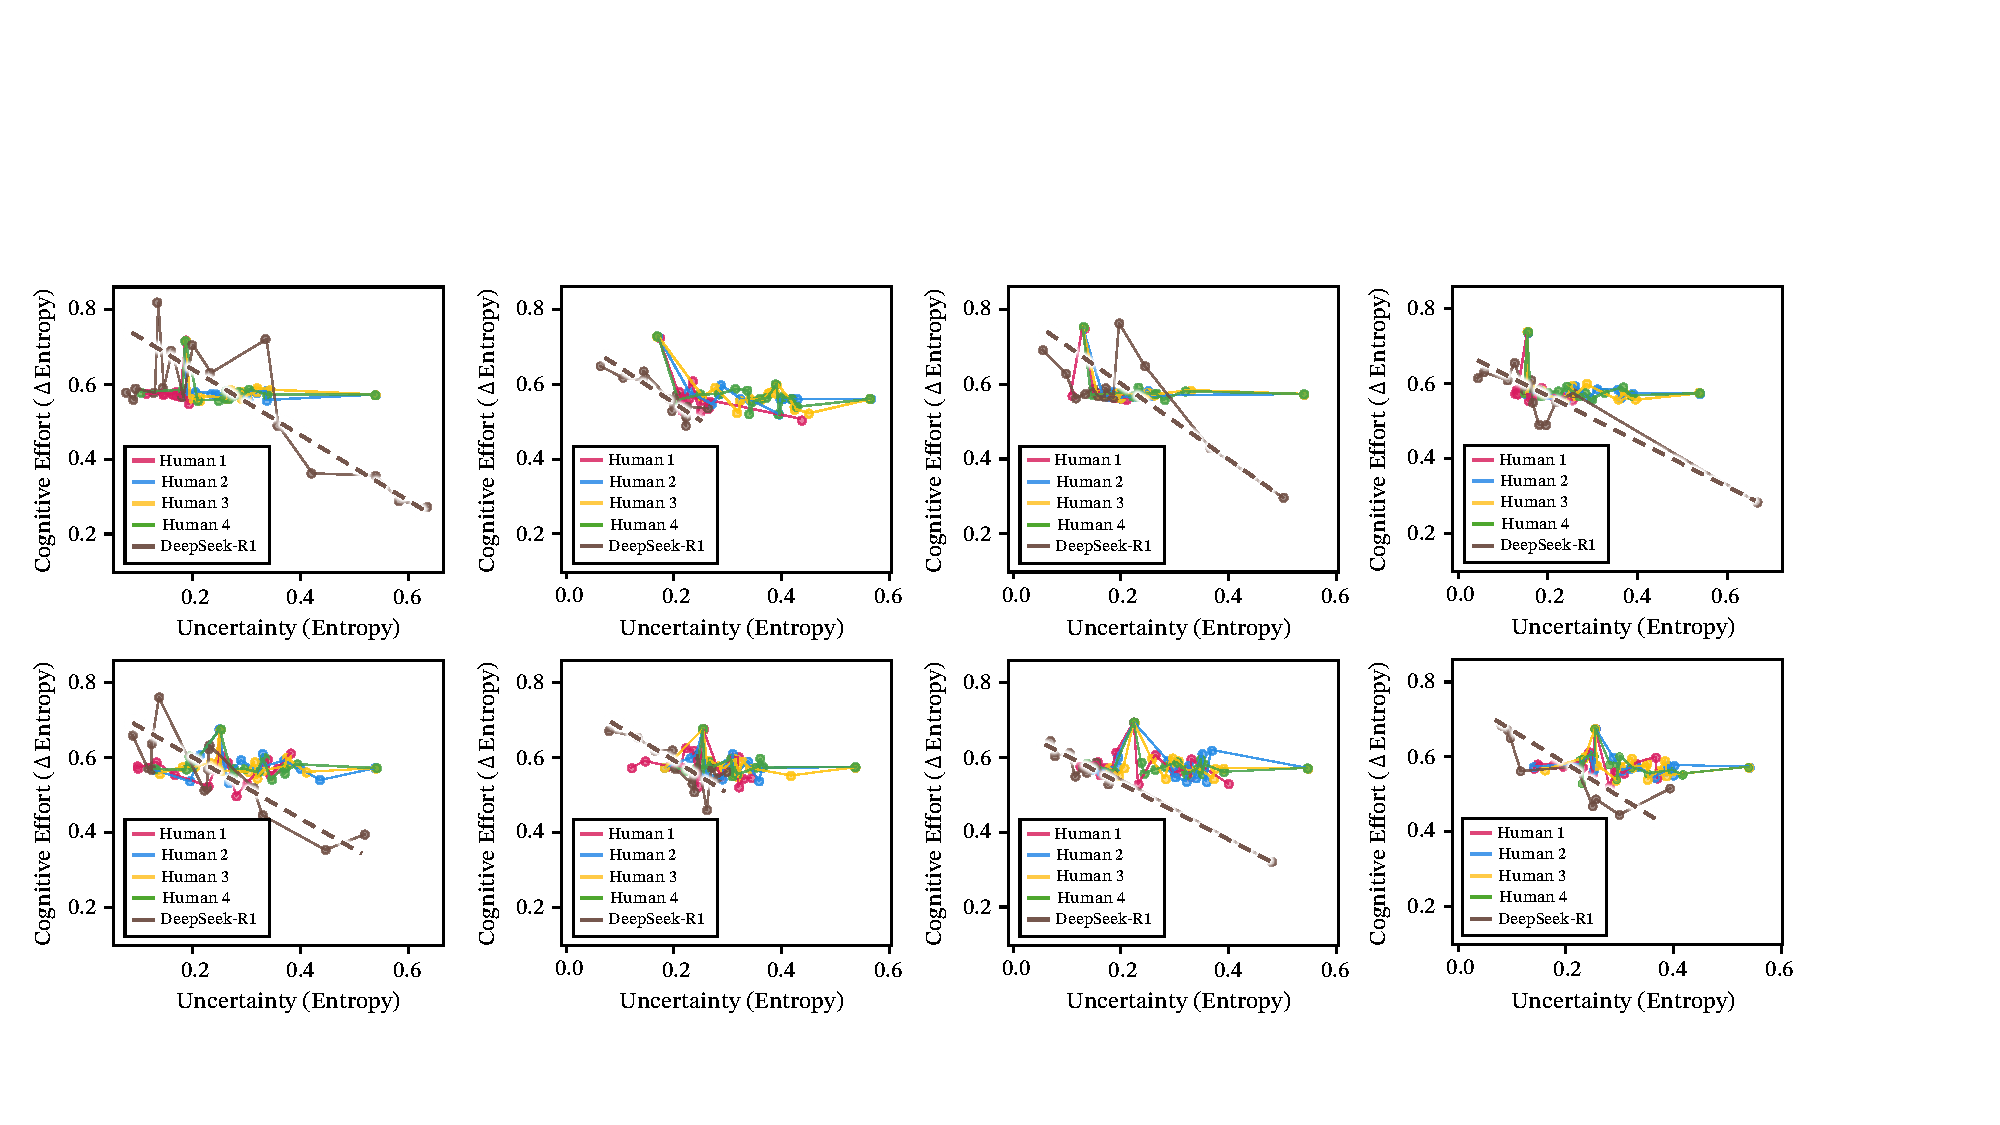
\includegraphics[width=\textwidth]{figures/effect-full.pdf}
    \caption{Information flow analysis for humans and reasoning models.}
    \label{fig:effect}
\end{figure*}


\begin{figure*}[t]
    \centering
    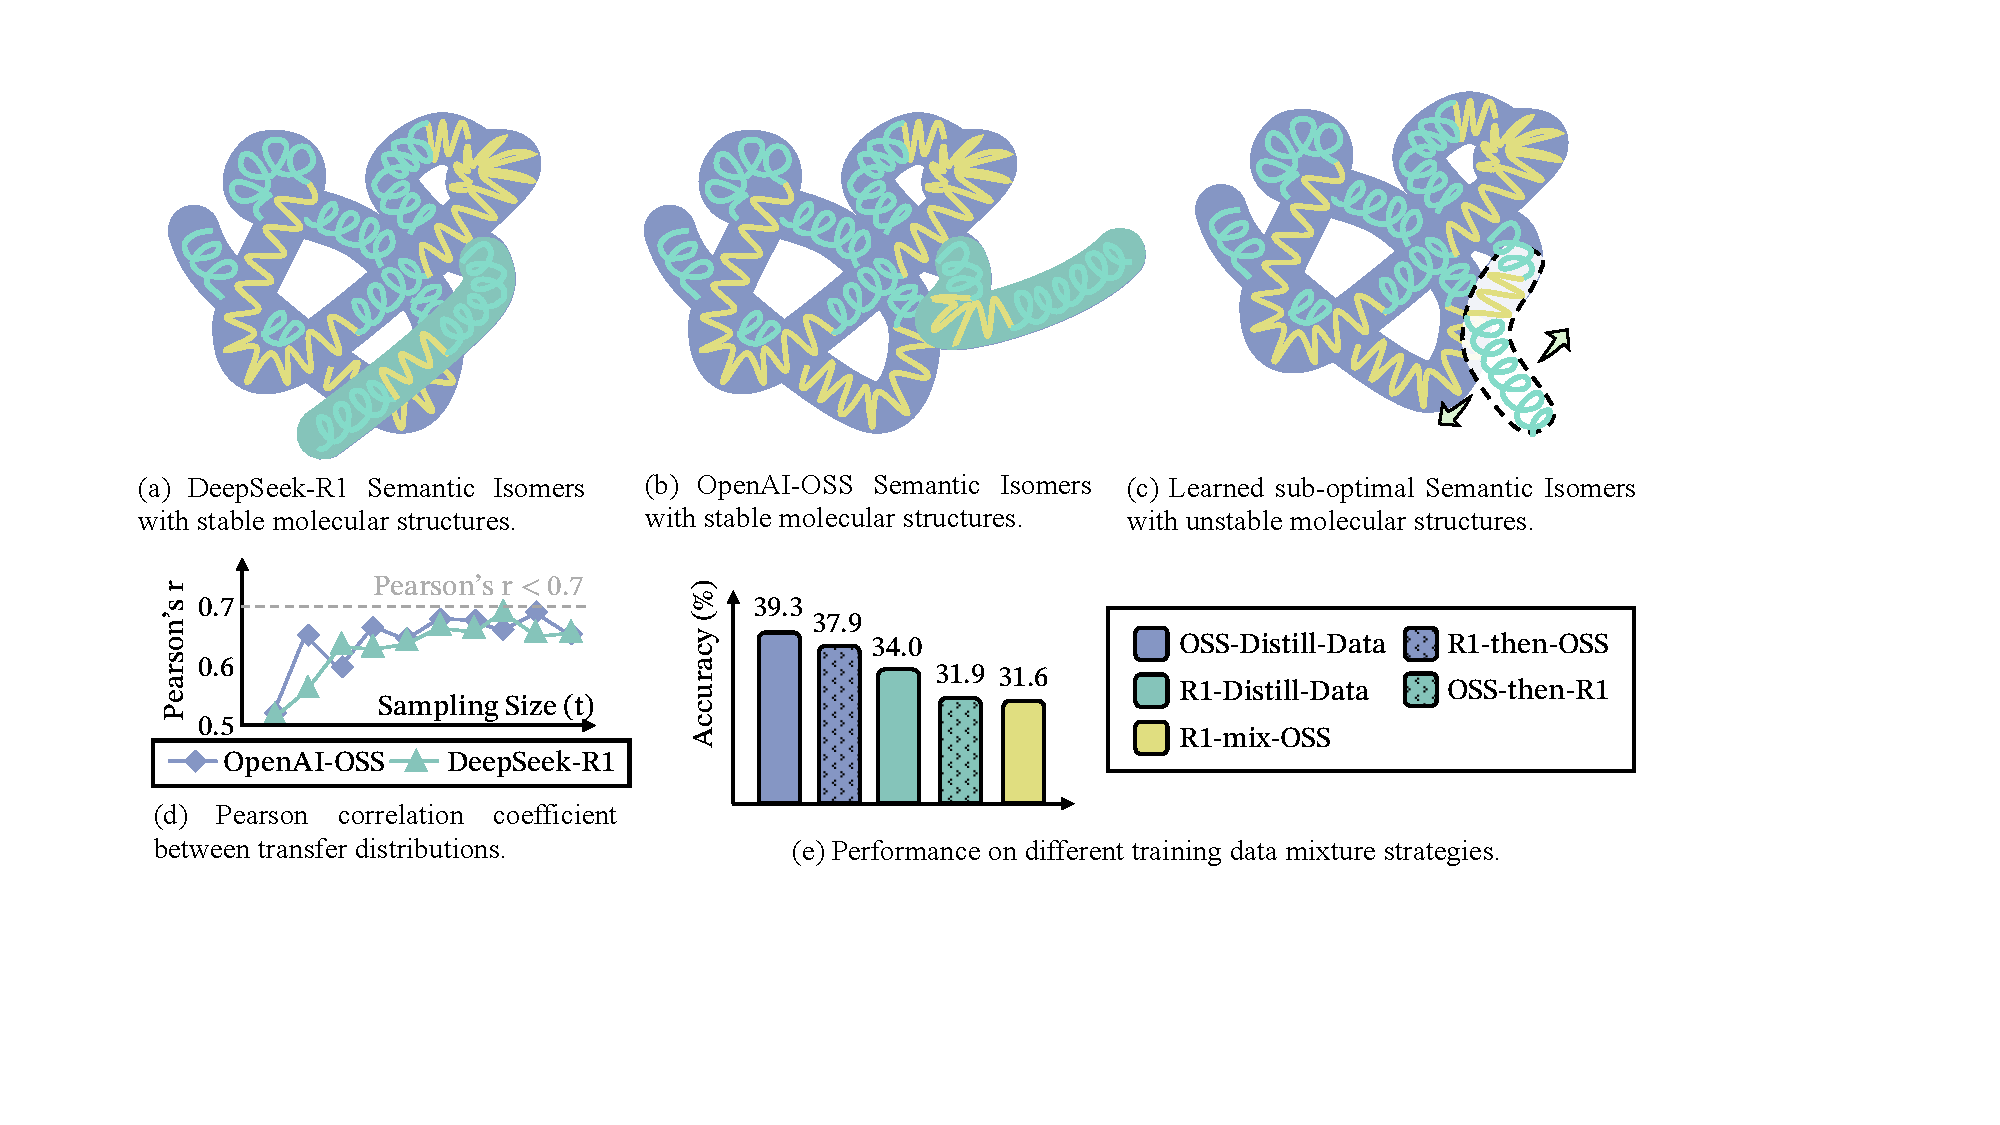
\includegraphics[width=0.98\textwidth]{figures/conflict.pdf}
    \caption{Conflict Learning between Two Stable Molecular Structures.}
    
    \label{fig:conflict}
\end{figure*}
\subsubsection{Not all bonds in isomers are effective.}

To clarify the nature of semantic isomers, we examine which bond structures yield effective reasoning configurations. We hypothesize that functional viability depends on specific bond distributions: despite sharing identical conceptual nodes, incompatible configurations disrupt information exchange. For instance, excessive exploration bonds cause fragmented reasoning, whereas overemphasized deep reasoning bonds create rigid chains unable to adapt to new inputs.Details are provided in Appendix~\ref{append:information}.\vspace{-8pt}


\paragraph{\textbf{Effective reasoning bond distribution influences the information divergence speed in reasoning dynamics.}}
To assess this, we compared the reasoning dynamics of R1 models with human cognition in an information phase space~\cite{chen2025universal}. Mechanistically, LLMs update by maximizing rewards and reducing entropy, whereas human reasoning is additionally constrained by semantic coherence and social feedback. Consequently, machine reasoning converges through accumulated gradient updates, whereas human reasoning stabilizes through iterative self-monitoring and social calibration.
As shown in Figure~\ref{fig:effect}, we tracked reasoning unfolding over extended chains in logical deduction tasks. Humans typically exhibit nearly uniform forward information gains (81.3\% of cases show changes $<0.1$), corresponding to a near-zero slope in phase space. In contrast, R1 models display accelerating informativeness (76.1\% of cases show absolute changes $>0.1$), progressing from low entropy to rapid convergence. These patterns indicate a fundamental difference in how R1 models and humans integrate information over time.\vspace{-8pt}


\paragraph{\textbf{Effective reasoning bonds cause metacognitive oscillation and alignment.}}
We identify the core rationale for this difference as a "metacognitive oscillation" in LLMs. Their responses alternate between high-entropy divergent exploration (slope \(> 0.6\), \(\Delta\)entropy \(> 0.05\)) and stable convergent validation, a dynamic less pronounced in the uniform entropy profiles of humans. Case studies (Figure~\ref{fig:effect}) confirm that R1 models utilize self-reflective revision to adjust reasoning paths against uncertainty. We hypothesize that aligning training objectives with these behavioral structure distributions can narrow the gap between machine and human reasoning dynamics.


\subsection{Conflict between Two Stable Structures}

Understanding how distinct reasoning structures interact reveals fundamental limits of complex cognitive systems. As shown in Fig.~\ref{fig:conflict} (a–c), forcibly fusing stable molecular isomers disrupts their backbone; analogously, combining incompatible reasoning frameworks breaks global logical coherence.\vspace{-8pt}

\paragraph{\textbf{Learning two heterogeneous stable structures at the same time will lead to structural chaos in the model.}}
As shown in Fig.~\ref{fig:conflict} (d), we test this by jointly activating two highly correlated (\(r \approx 0.9\)) reasoning chains from DeepSeek-R1 and OpenAI-OSS. Despite their similarity, co-activation prevents the model from converging to a single stable behavioral mode: it produces molecular bond distributions that fluctuate across samples and deviate from those characteristic of either OSS or R1. Consistent with this instability, the self-correlation of the jointly activated model does not exceed 0.8.\vspace{-8pt}

\paragraph{\textbf{This structural chaos leads to a significant decline in the performance of the model.}}
As shown in Fig.~\ref{fig:conflict} (e), joint activation also causes a marked drop in performance relative to either chain alone. This seemingly paradoxical effect indicates that structural compatibility, rather than mere statistical correlation, governs whether reasoning systems can coexist. The interference pattern suggests that the underlying cognitive architecture is rigid: without careful alignment, attempts to merge such systems yield fragmented, low-utility outputs instead of enhanced capability.


\begin{TakeawayBox}{Takeaway 3}
\begin{itemize}[leftmargin=16pt, itemsep=0pt, topsep=0pt]
    \item Well-structured isomers perform effectively when their reasoning-key distributions align closely, but small structural shifts cause fragility and sharp performance losses.
    \item Co-activating incompatible reasoning structures induces structural chaos that breaks coherence and degrades performance, proving that statistical similarity does not guarantee compatibility.
\end{itemize} 
\end{TakeawayBox}
